Wenn eine Applikation entwickelt werden soll, ist die Wahl der richtigen Methode, Frameworks oder auch der Programmiersprache eine wichtige Entscheidung für das Projekt. Viele Entscheidungen können im Verlauf der Entwicklung noch einfach geändert werden, aber um eine derartige Entscheidung zu ändern, müssen Teile der Anwendung oder auch der komplette Quellcode neu geschrieben werden. Dazu kommen tausende Artikel, warum die eine neue Programmiersprache der neue Standard ist. So ist eine derartig wichtige Entscheidung oft sehr schwierig.

Da oft Anwendungen nicht nur auf einem Gerätetyp laufen sollen, sondern allen Nutzern auf den verschiedensten Plattformen zur Verfügung stehen soll, hat diese Entscheidung noch einmal eine größere Bedeutung, da sie auch eng verbunden mit den Kosten der Entwicklung und der Erfahrung durch den Nutzer ist.

In Zeiten der Heimcomputer und des stetig wachsenden Internets war der einfachste Weg , eine Webseite zu entwickeln, die über den Browser der genutzten Geräte aufgerufen werden konnte. Mit der Ära der Smartphones jedoch änderte sich das. So waren Webapplikationen oft nicht für die Nutzung an derartig kleinen Geräten mit einer Toucheingabe angepasst.

Die Nutzung von Smartphones öffnete außerdem die Tür, andere Funktionalitäten wie die Kamera, Bluetooth oder GPS-Daten zu nutzen. Deshalb wurden Applikationen oft mit Objectiv-C beziehungsweise Swift für iOS und Java, jedoch mittlerweile Kotlin für Android entwickelt. Mit deren Hilfe wurden native Anwendungen für das Smartphone entwickelt, die diese neuen mobilen Plattformen optimal ausnutzen konnten.

Durch den Wunsch nach einer Multi-Plattform Anwendung, also dass die App für mehrere Plattformen veröffentlicht werden soll, muss jedoch für jede Plattform eine eigene Applikationen in der jeweiligen Programmiersprache und Technologie geschrieben werden. Dadurch entsteht ein sehr hoher Aufwand und die Kosten multiplizieren sich mit der Zahl der abzudeckenden Plattform. Deswegen wurde bereits früh mit der Entwicklung von sogenannten Cross-Plattform Technologien gestartet, die es ermöglichen sollen, mit einem geteilten Code so viele Plattformen wie möglich abzudecken. So erschien 2008 etwa PhoneGap. Es war ein Open-Source Framework zur Entwicklung von hybriden mobilen Applikationen, die mit Hilfe von HTML, CSS und Javascript programmiert wurden. PhoneGap und sein Nachfolger Cordova waren einige Zeit auch sehr beliebt in diesem Bereich. 2019 hatten beide zusammen einen Marktanteil von knapp 40\% unter den Cross-Plattform Frameworks \cite{statist_CP_Framework}.

Dennoch werden viele Entwicklung immer noch nativ entwickelt. So ergab eine interne Untersuchung der Firma \verb|ScanBot SDK|\footnote{https://scanbot.io/de/blog/native-apps-vs-cross-platform/}, dass 2019 57\% ihrer Nutzer native Applikationen entwickelten, obwohl ihr Produkt ebenso für viele der gängigen Cross-Plattform Frameworks zur Verfügung steht. Außerdem kann in Blogposts von einigen größeren Unternehmen lesen, in dem sie erklären, wie sie versuchten eine  Cross-Plattform-Entwicklungen einzuführen, jedoch aus verschiedenen Gründen  wieder einstellten. So etwa auch Airbnb \cite{Airbnb_react_goals}. Sie nutzten das von Facebook mitentwickelte Framework React Native. 2019 hatte dieses Framework einen Marktanteil von 42\%. 
\break
Ihre Ziele waren einfach:
\begin{enumerate}
    \item Schnelleres entwickeln.
    \item Die gleiche Codequalität beibehalten.
    \item Nur noch eine Codebasis.
    \item Die Entwicklererfahrung verbessern.
\end{enumerate}
Jedoch traten während der Entwicklung einige technische Probleme auf, die dazu führten, dass sie ihre Ziele nicht einhalten konnten und 2018 wieder zu einem nativen Ansatz zurückkehrten.

Durch Beispiele wie dieses, waren und sind App-Entwickler oft skeptisch gegenüber derartigen Lösungen, da dies auch immer mit großen Änderungen und hohen Investitionen verbunden sind. Dennoch ist der Wille da und auch die Zahl der Cross-Plattform Entwicklungen nimmt in den letzten Jahren zu. So ergab die Untersuchung von \verb|ScanBot SDK|, dass 2021 58\% Cross-Plattform Lösungen nutzten. Auch eine Untersuchung von Jetbrains ergab, dass 2021 53\% aller App Entwickler derartige Technologien nutzen \cite{JetBrains_miscellaneous_2021}.

\begin{figure}[ht]
  \centering
  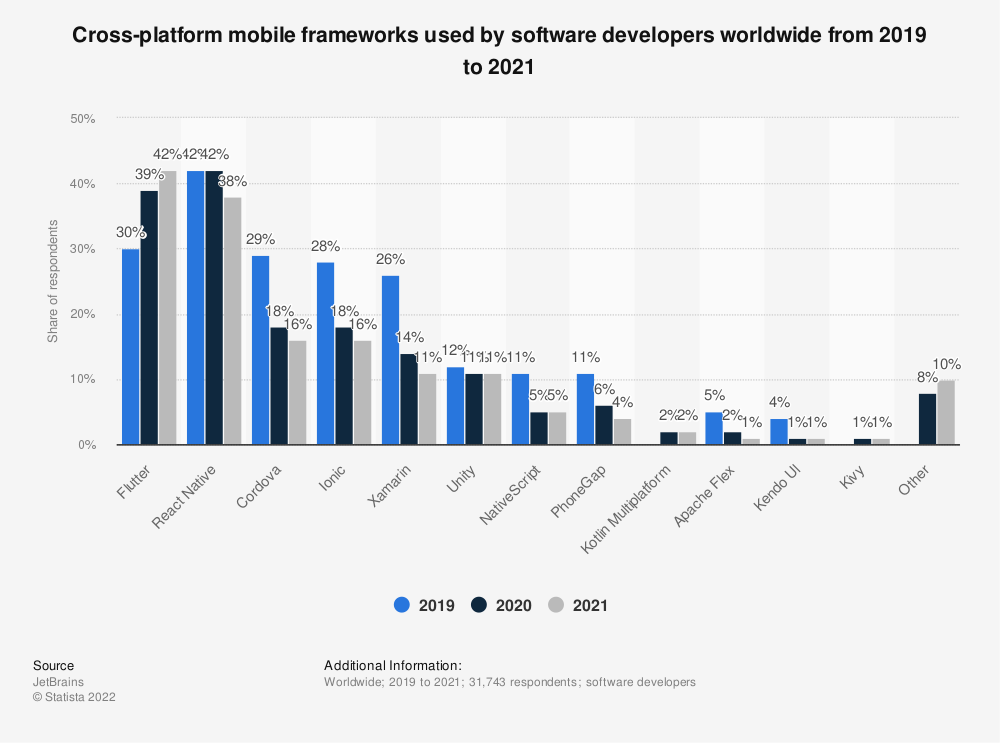
\includegraphics[height=7cm,keepaspectratio]{images/cross-platform-mobile-frameworks.png} 
  \caption[Statistik Cross-Plattform-Frameworks]{Cross-Plattform-Frameworks 2019-2021 \cite{statist_CP_Framework}}
  \label{fig:statista_cross_plattform}
\end{figure}

Diese Zahl könnte sich auch noch stark ändern. Abbildung \ref{fig:statista_cross_plattform} zeigt eine Statistik, die die Verteilung von verschiedenen Cross-Plattform-Entwicklungen zeigt. Sie zeigt eindrucksvoll wie schnell sich die Verteilung von Cross-Platform Frameworks ändern kann. Ein Framework, das hier jedoch besonders auffällt ist Flutter. Es ist ein Framework das erst 2017 auf den Markt gekommen ist und innerhalb von gerade einmal 4 Jahren auf einen Marktanteil von 42\% gekommen ist. Von einigen wird es als der neue Standard angesehen und viele Unternehmen steigen auf Flutter um oder bekunden großes Interesse daran. 

Jedoch gibt es auch Entwickler, die wegen Unsicherheiten und einigen anderen Gründen immer noch nativ entwickeln. So entwickelt die Number42 alle ihrer betreuten mobilen Applikationen mit den nativen Programmiersprachen. Auch die nativen Programmiersprachen entwickeln sich dabei stetig weiter und bekommen Änderungen, die eine Entwicklung vereinfachen und beschleunigen. Dadurch ist auch dieser Ansatz nicht von der Hand zu weisen und es kann durchaus sinnvoll sein, neue Apps weiterhin nativ zu entwickeln.

\section{Einordnung der Arbeit}
Diese Arbeit soll zunächst einen geordneten Überblick über die verschiedenen Entwicklungsansätze geben und somit eine gemeinsame Basis bilden, da es hier viele verschiedene Einordnungen gibt.
Danach soll anhand von verschiedenen Implementierungen eine Untersuchung von vier verschiedenen Ansätzen gemacht werden, um einige der vorgestellten Ansätze genauer zu betrachten.
Am Schluss soll anhand der verschiedenen Implementierungen und Erfahrungen während der Entwicklung ein Vergleich zwischen den ausgewählten Ansätzen gezogen werden und daraus ein Fragekatalog erstellt werden, der die Wahl eines passenden Ansatzes erleichtern soll.
Das Ziel der Arbeit ist es neben einer Vorstellung der verschiedene Ansätze zur Entwicklung von mobilen Anwendungen vor allem die Beispielhafte Untersuchung von vier Ansätzen anhand verschiedener Implementierungen sein. Dabei werden einige Grundlagen, benutzte Bibliotheken und einige Ergebnisse der Entwicklung vorgestellt werden. Danach wird anhand dieser Implementierungen und anderen Quellen ein Vergleich der aufgezeigten Ansätze gezogen werden. Dabei werden zuerst einige Faktoren verglichen und danach mit Hilfe gewählter Fragen und Erklärung ein Entscheidungskompass  erzeugt, der eine Auswahl eines Ansatzes erleichtern soll.
 
Diese Arbeit soll dabei vor allem eine genaue Einordnung von Entwicklungsansätzen bilden, da diese oft sehr unterschiedlich eingeteilt werden. Danach soll ein Vergleich angestellt werden um die unterschiedlichen Vor und Nachteile der untersuchten Ansätze vorzustellen. Dabei soll keine Aussage getroffen werden, welcher Ansatz der einzig richtige ist, sondern eher ein Leitfaden, um die richtige Technologie anhand der eigenen Gegebenheiten und Anforderungen zu treffen.

untersucht werden und einige Anhaltspunkte gegeben werden, um danach eine bessere Einschätzung treffen zu können, welcher Ansatz zur Programmierung von mobilen Anwendungen für den eigenen Einsatz geeignet ist. 
Neben einer geordneten Einordnung der verschiedenen Applikationsarten wird in dieser Arbeit vier verschiedene Ansätze genauer verglichen. Sie sollen dabei drei typische Arten der Entwicklung repräsentieren und noch eine vierte etwa experimentelle Mischimplementierung.
Dabei 


\section{Aufbau der Arbeit}
Diese Arbeit hat 6 Kapitel. Eine Einleitung und Motivation ist in Kapitel 1 zu finden. In Kapitel 2 werden verwandten Arbeiten vorgestellt, während in Kapitel 3 die verschiedenen App-Arten, das Projekt, die verschiedenen Implementierungen vorgestellt und eine Abgrenzung der Arbeit stattfindet.
Danach wird in Kapitel 4 die verschiedenen Implementierungen vorgestellt und einige Bemerkung zu der Entwicklung getroffen, dabei soll auch auf Stärken und Schwächen der einzelnen Implementierungen eingegangen werden, die bei der Implementierung aufgefallen sind.
In Kapitel 5 soll anschließend eine Auswertung der einzelnen Entwicklungsansätze stattfinden und anhand einiger Kriterien und weiterer Erklärungen Ein Vergleich gezogen werden. Zusätzlich wird anhand eines Fragenkatalogs mit Erklärungen ein Entscheidungskompass gegeben, der bei der Auswahl eines Ansatzes helfen soll.  Abschließend soll in Kapitel 6 ein Fazit gezogen werden und ein Ausblick auf künftige Arbeiten aufgezeigt werden.